\section{Segunda parte: amplificador no inversor}

Se arma el circuito de la fig. \ref{fig:2:esquema} en un \textit{protoboard}
con $R_1 = \SI{10}{\kilo\ohm}$ y $R_2 = \SI{15}{\kilo\ohm}$, un TL072 como
amplificador operacional y una fuente partida de $\SI{14}{\volt}$
alimentándolo, además de una pila de \SI{9}{\volt} como $V_1$.
Luego se utilizan distintos valores de resistencia $R_L$
(47, 10 y \SI{1}{\kilo\ohm}) y se miden las tensiones $v_i$ y $v_o$ para
calcular la ganancia del circuito.

Hecho esto, se modifica el circuito para convertirlo en el seguidor de tensión
de la fig. \ref{fig:2:esquema-seguidor} (ver sección
\ref{sec:intro:opamp-noinversor}) y se vuelven a utilizar los
mismos valores de $R_L$ para hallar los distintos puntos de trabajo.

\begin{figure}[H]
    \centering
    \begin{subfigure}[b]{0.45\textwidth}
        \centering
        \begin{circuitikz}
    \node[op amp] at (0, 0) (opamp) {};

    \draw(opamp.+) -- ++(-0.2, 0) node[label={left:$v_+ = v_i$}]{}
    to[battery1, a=$V_1$] ++(0, -2) coordinate(cg)
    node[ground]{};

    \draw(opamp.-) -- ++(-0.7, 0) node[label={above:$v_-$}]{}
    to[R, a=$R_1$] ++(-1.5, 0)
    to[short] ++(-0.2, 0) coordinate(ci)
    to[short] (cg -| ci) node[ground]{};

    \draw(opamp.-) -- ++(-0.2, 0)
    to[short, *-] ++(0, 2)
    to[R=$R_2$] ++(2.8, 0) coordinate(co)
    to[short] (opamp.out -| co) coordinate(co1) -- (opamp.out);

    \draw(co1) 
    to[short, *-o] ++(0.4, 0) node[right]{$v_o$};

    \draw(co1)
    to[R=$R_L$] (cg -| co1) node[ground]{};

    \draw(opamp.up) -- ++(0, 0.2) node[vcc]{$+V_{cc}$};
    \draw(opamp.down) -- ++(0, -0.2) node[vee]{$-V_{cc}$};
\end{circuitikz}

        \caption{Amplificador no inversor}
        \label{fig:2:esquema}
    \end{subfigure}
    \hfill
    \begin{subfigure}[b]{0.45\textwidth}
        \centering
        \begin{circuitikz}
    \node[op amp] at (0, 0) (opamp) {};

    \draw(opamp.+) -- ++(-0.2, 0) node[label={below:$v_+$}]{}
    to[R=$R_1$] ++(-2, 0) node[label={above:$v_i$}]{}
    to[battery1, a=$V_1$] ++(0, -2) coordinate(cg)
    node[ground]{};

    \draw(opamp.-) node[label={left:$v_-$}]{};

    \draw(opamp.-) -- ++(-0.2, 0)
    to[short] ++(0, 2)
    to[R=$R_2$] ++(2.8, 0) coordinate(co)
    to[short] (opamp.out -| co) coordinate(co1) -- (opamp.out);

    \draw(co1) 
    to[short, *-o] ++(0.4, 0) node[right]{$v_o$};

    \draw(co1)
    to[R=$R_L$] (cg -| co1) node[ground]{};

    \draw(opamp.up) -- ++(0, 0.2) node[vcc]{$+V_{cc}$};
    \draw(opamp.down) -- ++(0, -0.2) node[vee]{$-V_{cc}$};
\end{circuitikz}

        \caption{Amplificador seguidor de tensión}
        \label{fig:2:esquema-seguidor}
    \end{subfigure}
    \caption{Circuitos a implementar}
\end{figure}

\subsection{Resolución teórica}

El circuito de la fig. \ref{fig:2:esquema} es prácticamente idéntico al de
la fig. \ref{fig:intro:opamp-no-inversor}, con el agregado del resistor $R_L$
que no modifica el valor de la tensión de salida.

Si se utiliza el modelo ideal planteado en la sección
\ref{sec:intro}, se puede despreciar el efecto del resistor
$R_1$ en el circuito de la fig. \ref{fig:2:esquema-seguidor}, ya que no
circulará corriente por esta rama debido a la alta resistencia de entrada del
operacional. De esta forma se obtiene el mismo circuito de la fig.
\ref{fig:intro:opamp-no-inversor}, con resistencia infinita entre la terminal
inversora y masa.

Para ambos casos, entonces, se puede utilizar la ec.
\ref{ec:intro:opamp-noinversor}. Al propagar el error se obtiene nuevamente
la ec. \ref{ec:1-teoria:err-ganancia}, motivo por el cual se obtiene una 
ganancia $A = \num{2.5 \pm 0.15}$ para el caso del amplificador no inversor,
y $A = \num{1.0}$ para el seguidor de tensión (incertidumbre nula, puesto que
$R_1 = \infty$).


\newpage
\subsection{Simulación con LTSpice}

La simulación de LTSpice de la fig. \ref{fig:2:ltspice} del amplificador no
inversor de la fig. \ref{fig:2:esquema} arrojó una ganancia $A = 2.304$ en
todos los casos, que concuerda con el análisis teórico. El único factor que
varió fue la corriente $I_{R_L}$, de $0.4413$, $2.074$ y
$\SI{20.74}{\milli\ampere}$ para las resistencias de $47$, $10$ y 
$\SI{1}{\kilo\ohm}$.

Para el amplificador seguidor de tensión se simuló el circuito de la fig.
\ref{fig:2:esquema-seguidor} con LTSpice, según lo indicado en la fig.
\ref{fig:2:ltspice-seguidor}. En todos los casos se obtuvo una ganancia $A=0.998$, que
concuerda con lo visto en la sección anterior. La única variable que presentó
diferencias según el valor de $R_L$ que se utilizara fue, por supuesto, la 
corriente por dicho resistor, de $0.1911$, $0.8984$ y
$\SI{8.984}{\milli\ampere}$ para resistencias de $47$, $10$ y
$\SI{1}{\kilo\ohm}$, respectivamente.

\begin{figure}[H]
    \centering
    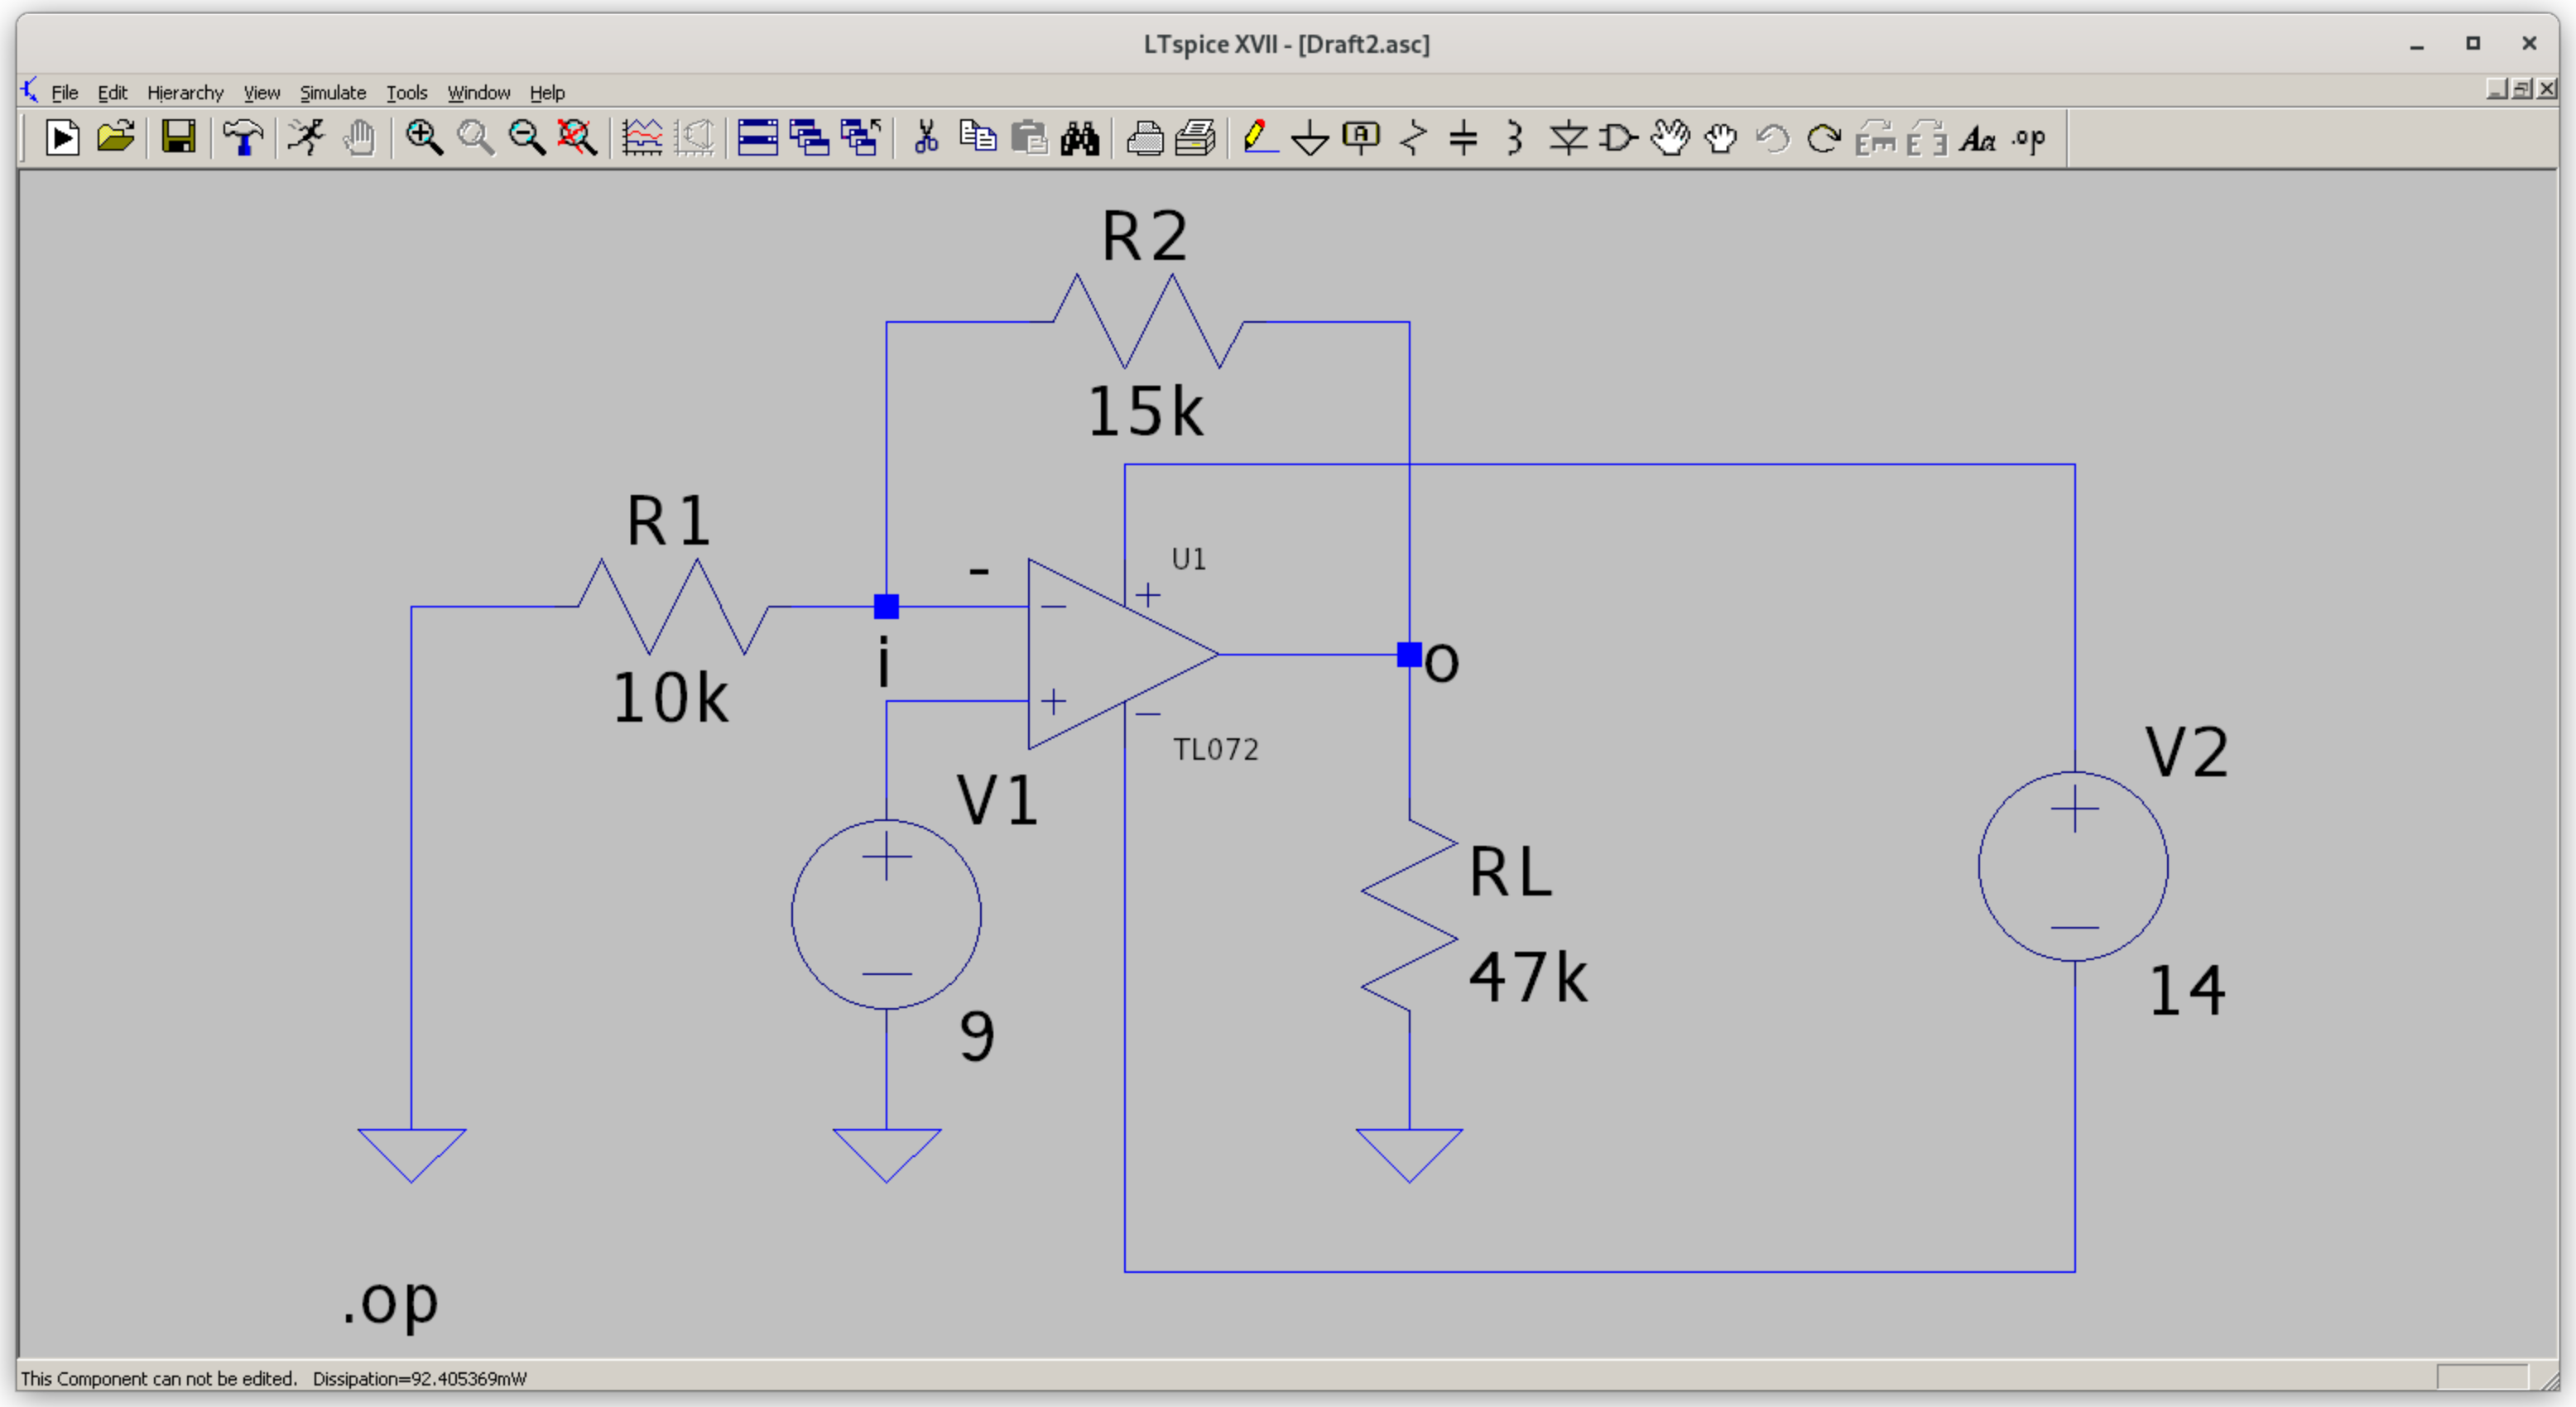
\includegraphics[width=0.8\textwidth]{img/2/ltspice.png}
    \caption{Simulación en LTSpice del circuito de la fig. \ref{fig:2:esquema}}
    \label{fig:2:ltspice}
\end{figure}

\begin{figure}[H]
    \centering
    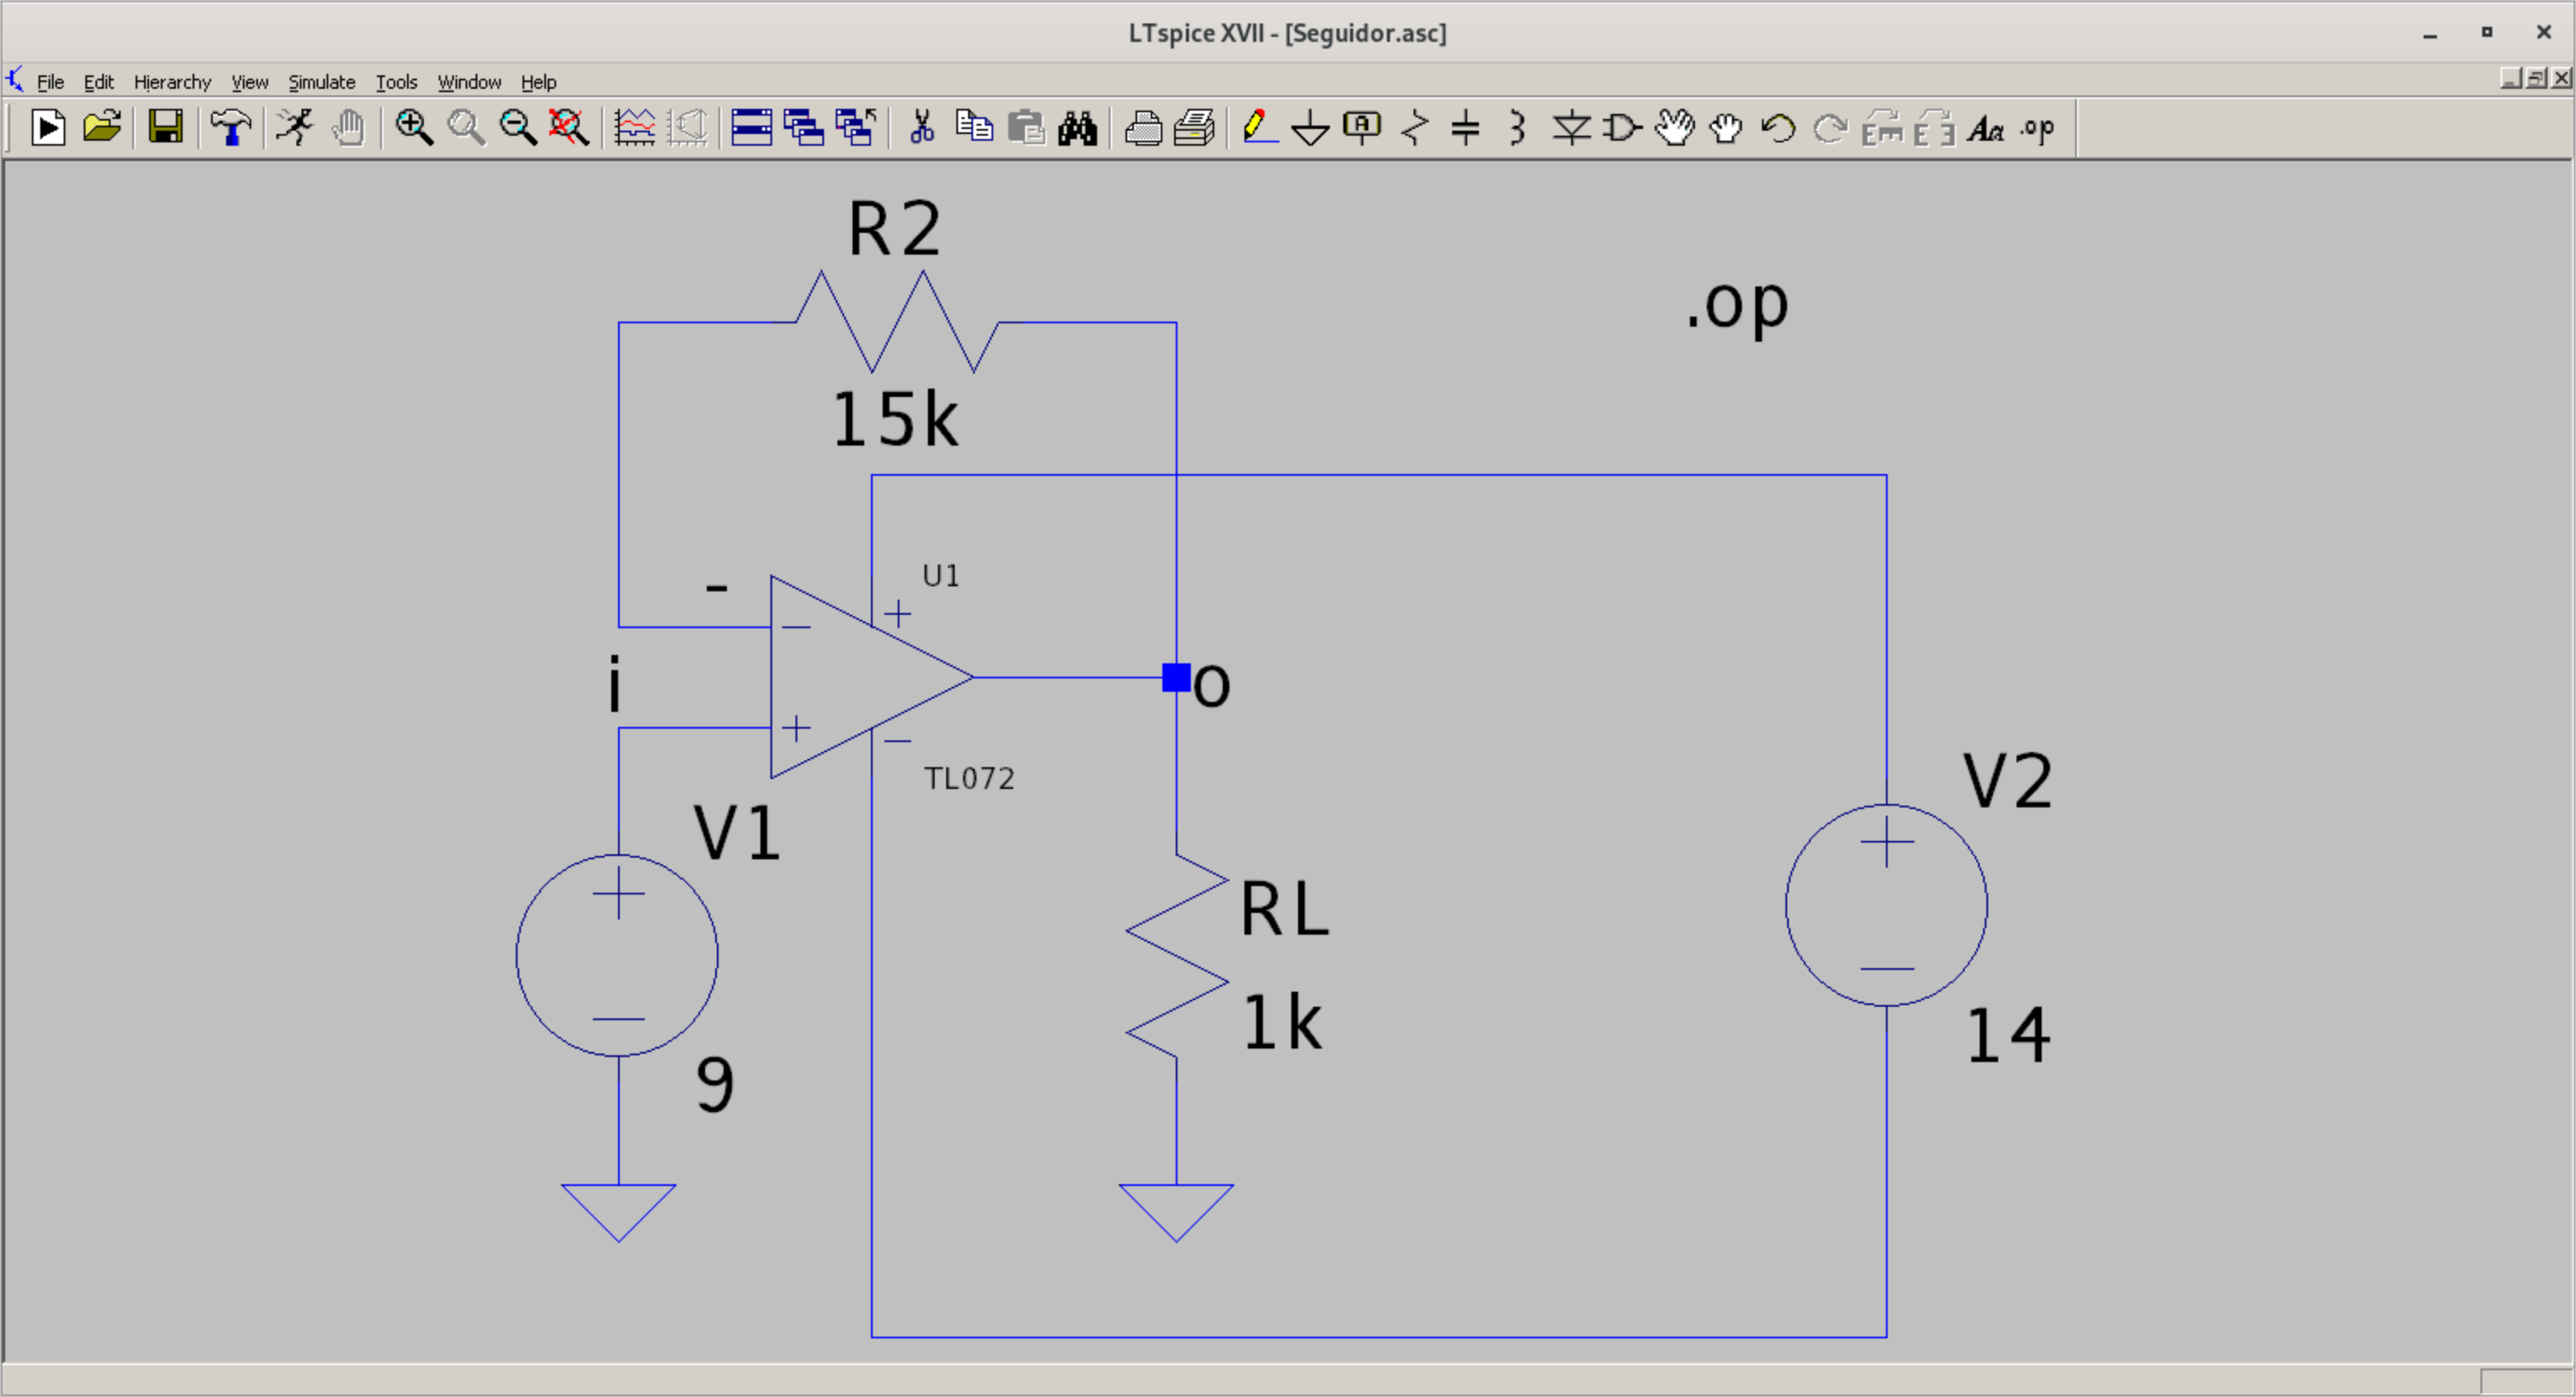
\includegraphics[width=0.8\textwidth]{img/2/ltspice-seguidor.png}
    \caption{Simulación en LTSpice del circuito de la fig.
        \ref{fig:2:esquema-seguidor}}
    \label{fig:2:ltspice-seguidor}
\end{figure}


\subsection{Datos obtenidos}

Para el amplificador no inversor, la tensión del nodo de entrada fue
$v_i = \SI{9.61 \pm 0.01}{\volt}$. Para los valores de resistencia 
$R_L$ de 47, 10 y \SI{1}{\kilo\ohm} se obtuvo siempre el mismo valor de
tensión a la salida del operacional: $v_o = \SI{20.90 \pm 0.01}{\volt}$.

Haciendo uso nuevamente de las ecuaciones \ref{ec:1-teoria:ganancia-experimental} y 
\ref{ec:1-teoria:err-ganancia-experimental} para el cálculo de la ganancia y del error, se
obtiene una ganancia $A = \num{2.174817898 \pm 0.003303660664}$.

En el caso del seguidor de tensión, $v_i = \SI{9.59 \pm 0.01}{\volt}$
y la salida registró $v_o = \SI{9.57 \pm 0.01}{\volt}$ para los tres valores
utilizados de $R_L$. La ganancia entonces es 
$A = \num{0.9979144943 \pm 0.002083331068}$.

Con los datos anteriores y sabiendo que

\[
    I_{R_L} = \frac{v_o}{R_L} \quad\quad
    \Delta I_{R_L} = \frac{\Delta v_o}{R_L} + 
                     \left| \frac{-v_o}{{R_L}^2} \right| \Delta R_L 
\]
se calculan los valores de la tabla \ref{tab:2-datos:irl}.

\begin{table}[H]
    \centering
    \begin{tabular}{@{}r|rr@{}}
        \toprule
        $R_L$ (nominal, \si{\kilo\ohm}) & $R_L$ (medido, \si{\kilo\ohm}) & $I_{R_L}$
            (\si{\micro\ampere}) \\
        \midrule
        47 & \num{46.6 \pm 0.1} & \num{205.4 \pm 0.7} \\
        10 & \num{15.64 \pm 0.01} & \num{612 \pm 1} \\
         1 & \num{9.94 \pm 0.01} & \num{963 \pm 2} \\ \bottomrule
    \end{tabular}
    \caption{Corrientes por las resistencias $R_L$ en el seguidor de tensión
    ($v_i = \SI{9.57 \pm 0.01}{\volt}$)}
    \label{tab:2-datos:irl}
\end{table}


\newpage
\subsection{Análisis de datos}

\begin{figure}[H]
    \centering
    \input{img/2/ganancia.tikz}
    \caption{Ganancia del amplificador no inversor}
    \label{fig:2-analisis:ganancia-opamp}
\end{figure}

\begin{figure}[H]
    \centering
    \input{img/2/ganancia-seguidor.tikz}
    \caption{Ganancia del seguidor de tensión}
    \label{fig:2-analisis:ganancia-seguidor}
\end{figure}

